%----------------------------------------------------------------------------
\chapter{Implementation}
%----------------------------------------------------------------------------
\section{Different versions of NI LabVIEW}
At the time of writing this thesis, National Instruments offers two versions of LabVIEW: LabVIEW 2018\footnote{\url{http://www.ni.com/en-us/shop/labview/labview-details.html}}, and LabVIEW NXG\footnote{\url{http://www.ni.com/en-us/shop/labview/labview-nxg.html}}. LabVIEW 2018 is a sequel to the LabVIEW versions released in the past few years, it operates reliably and fast, has support for all the NI hardware, and has a wide range of features. LabVIEW NXG is a brand new product, it has been created from scratch, and has been developed according to current standards - optimized for the newest hardware and software, and a really comfortable UI. Most features are still beta however, or under development\footnote{\url{http://www.ni.com/pdf/products/us/labview-roadmap.pdf}}, a large number of hardware are not yet supported, and the operation is not as reliable as the current generation software.\cite{nxg_article}

LabVIEW 2018 and LabVIEW NXG are not really compatible with each other, though the interface and the programming is similar, they have completely different execution engines and file formats. There is a tool bundled with NXG for current generation project conversion, but it is not perfect, and almost always the converted VIs need manual fixing afterwards.

Given two distinct LabVIEW products, it has to be decided which to develop the tool for. Both of them have advantages: current generation LabVIEW has a larger user base than NXG, but developing for NXG will make the tool compatible with actual software for a longer time (since NXG will eventually replace current generation LabVIEW).
\subsection{Comparing the API}
For making a decision on the LabVIEW version, the main point was the method of integrating the tool into LabVIEW. 

Reading the VI data from file is quite difficult. The file format definition of current generation VIs is not published, so the only software that can read the file is LabVIEW. NXG stores the VI data in XML files, which is a lot friendlier. It is possible to create an interpreter, and build the object model, since the nodes are XML elements, and the connections are made using unique identifiers.

Building a plugin is an option too. LabVIEW 2018 has a toolbox called VI Scripting\footnote{\url{http://sine.ni.com/nips/cds/view/p/lang/en/nid/209110}} for G language. It has several commands to access or modify VI object models and project structure. Project Provider Framework\footnote{\url{http://www.ni.com/white-paper/13921/en/}} allows an add-on to be integrated into the interface of LabVIEW, like creating a menu command or a toolbar button.

A plugin for LabVIEW NXG needs a different approach. Most of NXG uses .NET framework, and an add-on integrates in a form of a .NET class library (DLL). The object model of a Virtual Instrument is directly accessible as a .NET object, and plugin entry points can easily be defined with class attributes. UI elements can be easily created as well. This way, the plugin is written in C\# language.

I have chosen to create an NXG plugin, since writing such a complex tool in G language would require such an expertise in LabVIEW, that I do not have. Additionally, I already had the routine in NXG API and C\#.
\section{LabVIEW NXG API and object model}
There is hardly any documentation on the NXG programming interface at the moment, but an example plugin project on GitHub\footnote{\url{https://github.com/ni/nidevlabs}}. Fortunately, this project had almost all the API I needed for this project.
\lstset{escapechar=@}
\begin{lstlisting}[frame=single,escapechar=@,float=!ht,caption={The same program using a procedural paradigm},captionpos=b,label={lst:menuapi},language=C++]
[ExportPushCommandContent]
public class LauncherCommands : PushCommandContent
{
    public static readonly ICommandEx SymbolicMenuRoot = new RelayCommandEx(RelayCommandEx.HandleNoOp)
    {
        UniqueId = "SymbolicTool.MenuRoot",
        LabelTitle = "SymbolicTool",
        MenuParent = MenuPathCommands.RootMenu
    };
    public readonly ICommandEx RunCommand = new ShellRelayCommand(OnRun)
    {
        UniqueId = "SymbolicTool.RunCommand",
        LabelTitle = "Run Symbolic Execution",
        MenuParent = SymbolicMenuRoot
    };
    public override void CreateApplicationContent(ICommandPresentationContext context)
    {
        base.CreateApplicationContent(context);
        context.Add(SymbolicMenuRoot);
        context.Add(RunCommand);
    }
    public static void OnRun(ICommandParameter parameter, ICompositionHost host, DocumentEditSite site)
    {
    	* Run the program here *
    }
}
\end{lstlisting}

\begin{figure}

\centering
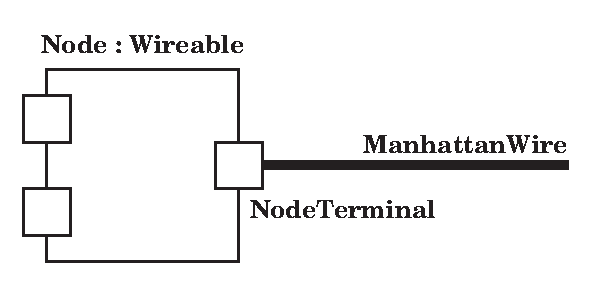
\includegraphics[width=80mm,keepaspectratio]{figures/lvobject.pdf}
\caption{LabVIEW Node object model} 
\label{fig:lvobject}
\end{figure}
I implemented a launcher code based on the ExamplePlugins project, that integrates a menu command into the menu bar of NXG (Listing \ref{lst:menuapi}). The three parameters of the callback function provide access to the object model of LabVIEW. DocumentEditSite refers to the currently opened document, and since the execution will run on the opened VI, getting the model will be really easy: \lstinline[columns=fixed]{rootElement = site.ActiveDocumentEditor?.EditorInfo?.RootElement;}

